%%%%%%%%%%%%%%%%%%%%%%%%%%%%%%%%%%%%%%%%%%%%%%%%%%%%%%%%%%%%%%%%%%%%%%%%%%%%%%%%
%2345678901234567890123456789012345678901234567890123456789012345678901234567890
%        1         2         3         4         5         6         7         8

\documentclass[letterpaper, 10 pt, conference]{ieeeconf}  % Comment this line out
                                                          % if you need a4paper
%\documentclass[a4paper, 10pt, conference]{ieeeconf}      % Use this line for a4
                                                          % paper

\IEEEoverridecommandlockouts                              % This command is only
                                                          % needed if you want to
                                                          % use the \thanks command
\overrideIEEEmargins
% See the \addtolength command later in the file to balance the column lengths
% on the last page of the document

\usepackage[utf8]{inputenc}
\usepackage[T1]{fontenc}
\usepackage{graphicx}
\usepackage{hyperref}
%\usepackage[subtle]{savetrees}

% The following packages can be found on http:\\www.ctan.org
%\usepackage{graphics} % for pdf, bitmapped graphics files
%\usepackage{epsfig} % for postscript graphics files
%\usepackage{mathptmx} % assumes new font selection scheme installed
%\usepackage{mathptmx} % assumes new font selection scheme installed
%\usepackage{amsmath} % assumes amsmath package installed
%\usepackage{amssymb}  % assumes amsmath package installed

\title{\LARGE \bf
Conduit: A C++ Library for Best-Effort High Performance Computing
}

\author{ \parbox{7 in}{\centering Matthew Andres Moreno, Santiago Rodriguez Papa, and Charles Ofria\\
        % \thanks{*Use the $\backslash$thanks command to put information here}\\
        Department of Computer Science and Engineering at Michigan State University\\
        {\tt\small mmore500@msu.edu}} 
        % \hspace*{ 0.5 in}
        % \parbox{3 in}{ \centering Pradeep Misra**
        % \thanks{**The footnote marks may be inserted manually}\\
        % Department of Electrical Engineering \\
        % Wright State University\\
        % Dayton, OH 45435, USA\\
        % {\tt\small pmisra@cs.wright.edu}}
}

% \author{Matthew Andres Moreno$^{1}$ and Pradeep Misra$^{2}$% <-this % stops a space
% \thanks{*This work was not supported by any organization}% <-this % stops a space
% \thanks{$^{1}$H. Kwakernaak is with Faculty of Electrical Engineering, Mathematics and Computer Science,
%         University of Twente, 7500 AE Enschede, The Netherlands
%         {\tt\small h.kwakernaak at papercept.net}}%
% \thanks{$^{2}$P. Misra is with the Department of Electrical Engineering, Wright State University,
%         Dayton, OH 45435, USA
%         {\tt\small p.misra at ieee.org}}%
% }


\begin{document}


\maketitle
\thispagestyle{empty}
\pagestyle{empty}


%%%%%%%%%%%%%%%%%%%%%%%%%%%%%%%%%%%%%%%%%%%%%%%%%%%%%%%%%%%%%%%%%%%%%%%%%%%%%%%%
\begin{abstract}
Developing software to effectively take advantage of growth in parallel and distributed processing capacity poses significant challenges.
Best-effort computing models, which relax synchronization requirements, have been proposed as a strategy to overcome challenges harness high performance computing at extreme scale.  
Although many programming languages and frameworks aim to facilitate software development for high performance applications, existing prevalent tools do not expose an explicit best-effort interface.
The Conduit C++ Library aims to provide a convenient interface for best-effort inter-thread and inter-process communication.
Here, we describe the motivation, objectives, design, and implementation of the library.
\end{abstract}


\section{INTRODUCTION}

The parallel and distributed processing capacity of high-performance computing clusters continues to increase rapidly, promising to continue enabling profound scientific and industrial innovations \cite{gagliardi2019international}.    
Hardware advances afford great opportunity, but also pose a serious challenge: developing approaches to effectively harness it.

The Message Passing Interface (MPI) standard \cite{gropp1996high}, which exposes communication primitives directly to the end user, has long served as the dominant approach for building distributed computing applications.
Although its explicit, imperative nature enables precise control over execution, it also poses significant expense in terms of programability.
This programability cost manifests in terms of programmer productivity, programmer domain knowledge requirements, software quality, and performance tuning stymied by program brittleness \cite{gu2019comparative, tang2014mpi}.
In response to such concerns, task-based frameworks such as Charm++ \cite{kale1993charm++}, Legion \cite{bauer2012legion}, Cilk \cite{blumofe1996cilk}, and Threading Building Blocks (TBB) \cite{reinders2007intel} have arisen.
Under the task-based paradigm, the programmer describes the dependency relationships among computational tasks and associated data but relies on the framework runtime to automatically schedule and manage execution.
In a parallel vein, programming languages and extensions like Unified Parallel C (UPC) \cite{el2006upc} and Chapel \cite{chamberlain2007parallel} rely on on programmers to direct execution, but equips them with powerful abstractions, such as global shared memory.

In addition to programmability challenges, as HPC systems scale, deterministic algorithms depending on global synchronization become increasingly costly \cite{gropp2013programming,dongarra2014applied}.
Best-effort computing, where data dependencies are relaxed to reduce synchronization \cite{chakradhar2010best}, can improve scalability \cite{meng2009best}.
Algorithms performing a search or optimization with many acceptable results or employing pseudo-stochastic methods can, in cases, tolerate best-effort computing.
However, existing distributed computing frameworks do not explicitly expose a convenient best-effort interface.

The Conduit C++ Library aims to compliment the parallel and distributed programming ecosystem by exposing an explicitly best-effort, unsynchronized interface.
Under this interface, message dispatch or delivery may be preempted in favor of more recent messages, messages may be dropped under backlog conditions, and read operations may opt to view the most recently received message in lieu of blocking for receipt of an expected message.
(The library also provides an interoperable deterministic interface).
Conduit's implementation explicitly targets performant inter-thread and inter-process communication, utilizing lock-free operations for the former and providing automatic message pooling and aggregation for the latter.


\section{DESIGN APPROACH}

   \begin{figure}[thpb]
      \centering
      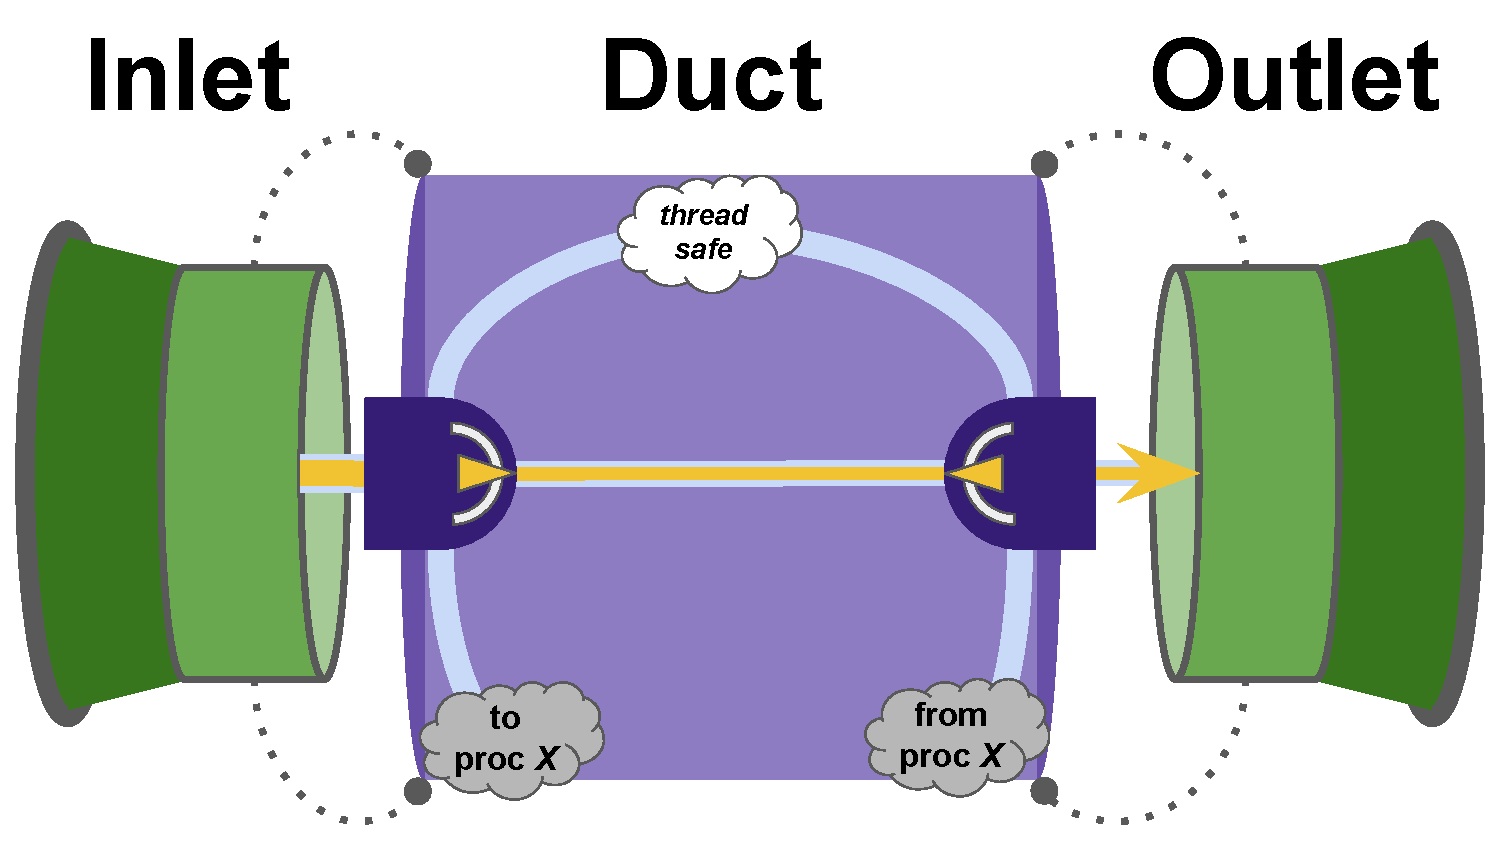
\includegraphics[width=0.8\linewidth]{img/conduit}
      \caption{Schematic of Conduit's \texttt{Inlet} and \texttt{Outlet} object scheme, where communication behavior is controlled, invisibly to the end-user, by an underlying \texttt{Duct} object.}
      \label{fig:conduit}
   \end{figure}

Conduit represents communication in terms of a paired \texttt{Inlet}, which accepts messages, and \texttt{Outlet}, which dispenses messages.
An \texttt{Inlet} and \texttt{Outlet} may exchange messages via an intra-thread, inter-thread, or inter-process communication procedure, depending on the runtime state of an underlying held \texttt{Duct} object.
Figure \ref{fig:conduit} provides a schematic overview.
The identity of which intra-thread, inter-thread, and inter-process implementation to rely on may be configured at compile-time.
Conduit provides a library of intra-thread, inter-thread, and inter-process implementations with different (i.e., best-effort or deterministic) properties to choose from.

The \texttt{Inlet} provides a non-blocking \texttt{TryPut()} method as well as a blocking \texttt{Put()} method.
The \texttt{Outlet} provides a \texttt{Get()} method to access the most-recently received message.
The next or latest message can be processed by \texttt{TryStep()} or \texttt{Jump()}, respectively.
A \texttt{Step()} method provides a blocking option to retrieve the next available message
At run time, \texttt{Duct}s can be created or modified to do intrathread, interthread, or interprocess communication. 

In addition to this granular connection-level interface, Conduit provides a network-level interface that enables the user to define a network topology, assign nodes in that topology to available threads across available processes, and automatically instantiate appropriate conduits.
Conduit provides several pre-defined topologies and node-assignment algorithms. 
Users can also opt to use the NetworkX graph library \cite{hagberg2008exploring} to generate arbitrary topologies and the METIS software package \cite{gupta1997fast} to automatically balance expected load across available threads and processes while minimizing inter-process and inter-thread communication.

\section{ IMPLEMENTATION }

Conduit's implementation has been developed around the following principles.

\begin{itemize}
    \item \textbf{overdecomposition}: Conduit provides a uniform API for intra-thread, inter-thread, and inter-process communication between agents.
    \item \textbf{testability}: Interchangeablility of inter-thread and inter-process communication for intra-thread communication makes software more readily unit-testable.
    \item \textbf{don't use what you don't want}: Multi-thread execution may be performed without MPI runtime.
    \item \textbf{don't pay for what you don't use}: Intra-thread, inter-thread, and inter-process communication are explicitly handled by separate, optimized implementations. 
    \item \textbf{modularity}: Different intra-thread, inter-thread, or inter-process implementations can be trivially interchanged for rapid prototyping and tuning.
    \item \textbf{flexibility}: Communication primitives may trivially rearranged to form arbitrary network structures. 
    \item \textbf{extensibility}: Users may provide communication implementations or network topologies.
    \item \textbf{lightweight}: The core components of Conduit are built as a header-only library.
    \item \textbf{portability}: Conduit is built using MPI and C++17 standards.
    \item \textbf{interoperability}: Conduit is compatible with other multithread and MPI code.
    \item \textbf{simplicity}: Conduit manages resource initialization and lifetime automatically.
    % \item \textbf{intuitiveness}: TODO object-oriented model with a simple API and an intuitive real-world analogy.
\end{itemize}

Source code is hosted on GitHub at \url{https://github.com/mmore500/conduit}, made freely available under a MIT License.
Documentation is hosted on ReadTheDocs at \url{https://conduit.fyi}.
A containerized build environment for Conduit is hosted on DockerHub at \url{https://hub.docker.com/r/mmore500/conduit}.

Conduit was built using the cereal C++11 Library for serialization \cite{voorhies2017cereal} and the Empirical C++ Library for Scientific Software \cite{charles_ofria_2019_2575607}.

%\section{Conclusion}

% The elements of real-time computing.

FIXING THIS PART

Necessity of Best-effort, unsynchronized 
The approach has been the open problem ``open-ended evolution'' within the artificial life community, a topic that has provoked long-term interest around defining, understanding the prerequisites and mechanisms of, and realizing the concept \cite{taylor2016open}.
Recent work has suggested that hardware compute constraints in existing systems meaningfully limit the of artificial life models to exhibit open-ended characteristics \cite{channon2019maximum}.
What a computational system that would allow for open-endedness, with Ackley suggesting a concept of ``indefinite scalability'' \cite{ackley2011pursue}.
Among other considerations, Ackley highlights the necessity of pursuing a best-effort, real-time paradigm in such a system. for reasons that you can't get synchronous to be good for arbitrarily big.



\addtolength{\textheight}{-12cm}   % This command serves to balance the column lengths
                                  % on the last page of the document manually. It shortens
                                  % the textheight of the last page by a suitable amount.
                                  % This command does not take effect until the next page
                                  % so it should come on the page before the last. Make
                                  % sure that you do not shorten the textheight too much.


\section*{ACKNOWLEDGEMENT}


Thanks to Katherine Perry for help with software development.
This research was supported in part by NSF grants DEB-1655715 and DBI-0939454, and by Michigan State University through the computational resources provided by the Institute for Cyber-Enabled Research.
This material is based upon work supported by the National Science Foundation Graduate Research Fellowship under Grant No. DGE-1424871.
Any opinions, findings, and conclusions or recommendations expressed in this material are those of the author(s) and do not necessarily reflect the views of the National Science Foundation.


%%%%%%%%%%%%%%%%%%%%%%%%%%%%%%%%%%%%%%%%%%%%%%%%%%%%%%%%%%%%%%%%%%%%%%%%%%%%%%%%

\bibliography{bibl}
\bibliographystyle{ieeetr}

\end{document}
